\providedisablepart{showscreenshot}
\begin{frame}
    \frametitle{Prover Generation}
    \begin{itemize}
        \item Can describe inference rules in MMT
        \item {\tt $\vdash$X} is the type of proofs of {\tt X}\com{``Judgments as types''}
        \item Example rules:\\
            {\boldmath\tt andEl \ : {\color{black!50}\{A,B\}} $\vdash\,$A$\wedge$B $\rightarrow$ $\vdash\,$A}\\
            {\boldmath\tt andEr \ : {\color{black!50}\{A,B\}} $\vdash\,$A$\wedge$B $\rightarrow$ $\vdash\,$B}\\
            {\boldmath\tt contra : {\color{black!50}\{X\}} $\vdash\,$male(X) $\rightarrow$ $\vdash\,$fem(X) $\rightarrow$ $\lightning$}
        \pause
        \item Generate Prolog/ELPI rules:\\
        {\boldmath\tt
provable(A) \ \ \ \ :- provable(A$\wedge$B).\\
provable(B) \ \ \ \ :- provable(A$\wedge$B).\\
contradiction() :- provable(male(X)), provable(fem(X)).\\
        }
        \item Extra predicates to guide proof search\com{iterative deepening, ...}
    \end{itemize}
    \ifpart{showscreenshot}{\only<3>{
        \begin{tikzpicture}[overlay,remember picture]
            \fill[gray!80,opacity=0.8] (current page.north west) rectangle (current page.south east);
            \node at (current page.center) { 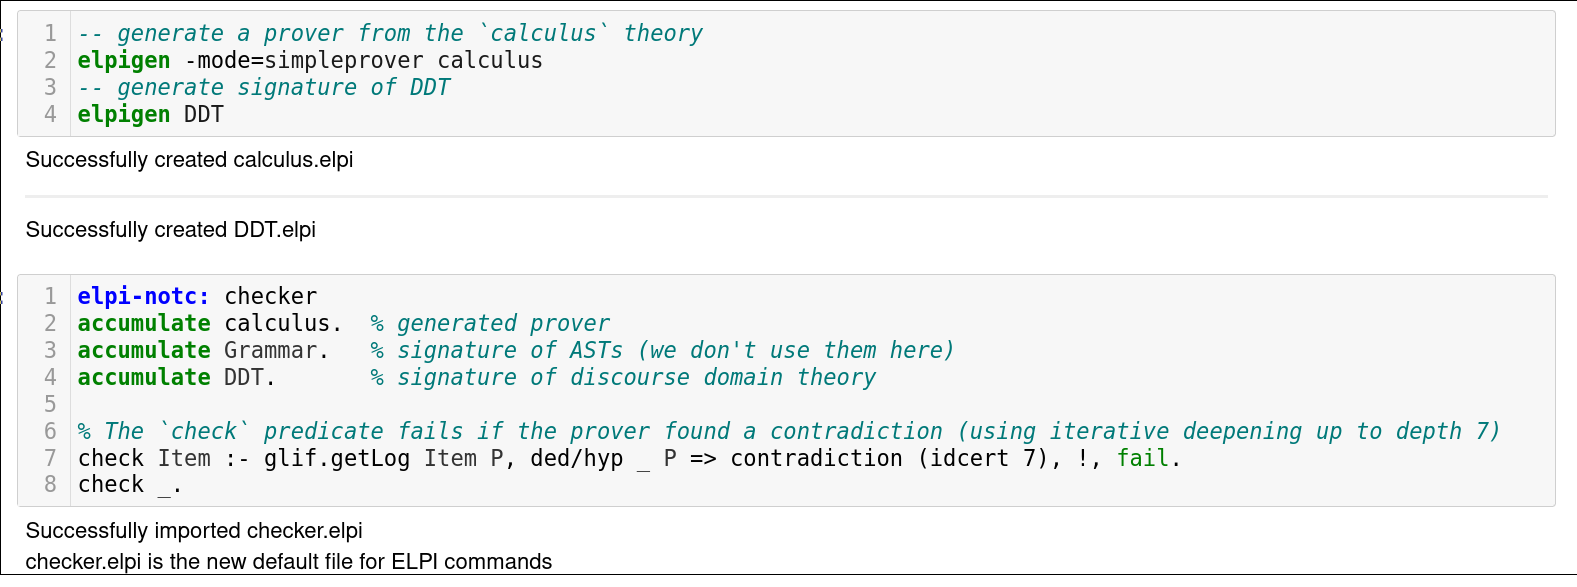
\includegraphics[width=0.95\textwidth]{img/screenshot-glif-6.png} };
        \end{tikzpicture}
    }}{}
\end{frame}
